\section{Latent Label Order in Multi-label Classification} \label{sec:2-1}

\subsection{Background}

Multi-label text classification is an important machine learning task wherein one must predict a set of labels to associate with a given document; for example, a news article might be tagged with labels \texttt{sport}, \texttt{football}, \texttt{2018 world cup}, and \texttt{Russia}. Formally, we are given a set of label candidates $\mathcal{L}=\{1,2,...,L\}$, and we aim to build a classifier which maps a document $x$ to a set of labels $\mathbf{y}\subset \mathcal{L}$. The label set $\mathbf{y}$ is typically written as a binary vector $\mathbf{y}\in \{0,1\}^L$, with each bit $y_{\ell}$ indicating the presence or absence of a label.

In multi-label prediction, labels often exhibit complex dependencies: knowing some labels---such as \texttt{sport} and \texttt{football}---should make it easier to predict \texttt{2018 world cup} and then \texttt{Russia}. There are several methods that manage to capture label dependencies by building a joint probability estimation over all labels $p(\mathbf{y}=(y_1,y_2,...,y_L)|x)$ \cite{ghamrawi2005collective,read2009classifier,DBLP:conf/icml/DembczynskiCH10,li2016conditional}. 
% \kechen{put BR before the introduction of dependency? because there is nothing about dependency by using BR} 
The most popular approach is to model multi-label prediction as a sequence prediction task. This is usually obtained by assigning the labels a globally fixed order (e.g.\ by label frequency), and learning labels one-by-one. In this way, the prediction of a single label is dependent on the prediction in the earlier sequence. Recently, RNNs become one of the most popular sequence prediction models, and have been applied to multi-label classification \cite{DBLP:conf/cvpr/WangYMHHX16,DBLP:journals/corr/ZhangWSZL16,DBLP:conf/icpr/JinN16,DBLP:conf/iccv/WangCLXL17,DBLP:journals/corr/abs-1709-08553,DBLP:conf/aaai/ChenCYW18,DBLP:journals/corr/abs-1806-04822}.  

To review how RNN can be used to solve a sequence prediction task, let $\mathbf{s}=(s_1,s_2,...,s_T)$ be an input sequence of outcomes, in a particular order, where $s_t \in \{1,2,...,L\}$; the order is often critical to the datapoint. An RNN model defines a probability distribution over all possible output sequences given the input in the form $p(\mathbf{s}=(s_1,s_2,...,s_T)|x)=\prod_{t=1}^T p(s_t|x,s_1,s_2,...,s_{t-1})$. To train the RNN model, one maximizes the likelihood of the ground truth sequence. %$p(\mathbf{s}=(s_1,s_2,...,s_T)|x)$.
At prediction time, one seeks to find the sequence with the highest probability $\mathbf{s}^*=\arg\max_\mathbf{s} p(\mathbf{s}|x)$, and this is usually implemented approximately with a beam search procedure \cite{lowerre1976harpy}. The sequence history is encoded with an internal memory vector $h_t$ which is updated over time. RNN is also often equipped with the attention mechanism \cite{DBLP:journals/corr/BahdanauCB14}, which in each timestep $t$ puts different weights on different words (features) and thus effectively attends on a list of important words. The context vector $c_t$ is computed as the weighted average over the dense representation of important words to capture information from the document. The context $c_t$, the RNN memory $h_t$ at timestep $t$, and the encoding of previous label ${s_{t-1}}$ are all concatenated and used to model the label probability distribution at time $t$ as $p(s_t|x,s_1,s_2,...,s_{t-1}) \sim \softmax(\phi(c_t,h_t,s_{t-1}))$, where $\phi$ is a non-linear function, and $\softmax$ is the normalized exponential function. RNN is trained with the standard maximum likelihood objective \cite{DBLP:conf/nips/NamMKF17}: 
\begin{align}
\maximize \sum_{n=1}^N \log p(\mathbf{s}^{(n)}|x^{(n)})
\label{eq:standard_rnn}
\end{align}
where $x^{(n)}$ is the $n$-th document and $N$ is the total number of documents in the corpus. 

One of the challenges of mapping a set to a sequence is to determine the appropriate label order. Vinyals \cite{vinyals2015order} proposes to dynamically choose during training the sequence order deemed as most probable by the current RNN model:
\begin{align}
\maximize \sum_{n=1}^N \max_{\mathbf{s}\in \pi(\mathbf{y}^{(n)})}\log p(\mathbf{s}|x^{(n)})
\label{eq:max_obj}
%\vspace{-2ex}
\end{align}
where the $\pi(\mathbf{y}^{(n)})$ stands for all permutations of the label set $\mathbf{y}^{(n)}$. This eliminates the need to manually specify the label order.
However, as noticed by the authors, this objective cannot be used in the early training stages: the early order choice (often random) is reinforced by this objective and can be stuck upon permanently. To address this issue, Vinyals \cite{vinyals2015order}~also proposes two smoother alternative objectives to initialize the model training:

The authors suggest that one first consider many random orders for each label set in order to explore the space:
\begin{align}
\maximize \sum_{n=1}^N \sum_{\mathbf{s}\in \pi(\mathbf{y}^{(n)})}\log p(\mathbf{s}|x^{(n)})
\label{eq:wrong_obj}
\end{align} 

After that, one can sample sequences following the model predictive distribution instead of uniform distribution:
\begin{align}
\maximize \sum_{n=1}^N \sum_{\mathbf{s}\in \pi(\mathbf{y}^{(n)})}p(\mathbf{s}|x^{(n)})\log p(\mathbf{s}|x^{(n)})
\label{eq:sample_obj}
\end{align} 

In training, one needs to schedule the transition among these objectives, a rather tricky endeavor. At prediction time, one needs to find the most probable set. This is done by (approximately) finding the most probable sequence $\mathbf{s}^*=\arg\max_\mathbf{s} p(\mathbf{s}|x)$ and treating it as a set $\hat{\mathbf{y}}=set(\mathbf{s}^*)$. With a large number of sequences, it is quite possible that the argmax has actually a low probability, which can lead to neglecting important information when we ignore sequences other than the top one.



\subsection{Decomposing Multi-label Set Prediction into Sequence Permutations Prediction}

We propose a new way of adapting RNN to multi-label set prediction, which we call \emph{set-RNN}. We appreciate the RNN model structure \cite{rumelhart1988learning} (defines a probability distribution over all possible sequences directly) and introduce training and prediction objectives tailored for sets that take advantage of it, while making a clear distinction between the sequence probability $p(\mathbf{s}|x)$ and the set probability $p(\mathbf{y}|x)$. 
 We define the set probability as the sum of sequences probabilities for all sequence permutations of the set, namely $p(\mathbf{y}|x)=\sum_{\mathbf{s}\in \pi(\mathbf{y})} p(\mathbf{s}|x)$. Based on this formulation, an RNN also defines a probability distribution over all possible sets indirectly since $\sum_{\mathbf{y}} p(\mathbf{y}|x)=\sum_{\mathbf{y}}\sum_{\mathbf{s}\in \pi(\mathbf{y})} p(\mathbf{s}|x)=\sum_{\mathbf{s}} p(\mathbf{s}|x)=1$. This formula can also be interpreted as a latent variable objective: $p(\mathbf{y}|x)=\sum_{\mathbf{s}\in \pi(\mathbf{y})} p(y|\mathbf{s})p(\mathbf{s}|x)$, where the label order $\mathbf{s}$ is seen as a latent variable and $\pi(\mathbf{y})$ is a set including all possible latent states. Because the process of mapping a sequence to a set does not contain any uncertainty, the probability $p(y|\mathbf{s})$ equals to 1. Then we can ignore this term from the latent variable objective. In standard maximum likelihood training, one wishes to maximize the likelihood of given label sets, namely, $\prod_{n=1}^N p(\mathbf{y}^{(n)}|x^{(n)})=\prod_{n=1}^N \sum_{\mathbf{s}\in \pi(\mathbf{y}^{(n)})} p(\mathbf{s}|x^{(n)})$, or equivalently, 
\begin{align}
\maximize \sum_{n=1}^N \log \sum_{\mathbf{s}\in \pi(\mathbf{y}^{(n)})} p(\mathbf{s}|x^{(n)})
\label{eq:right_obj}
\end{align}


%This training objective (\ref{eq:right_obj}) looks similar to the objective (\ref{eq:wrong_obj}) considered in previous work \cite{vinyals2015order}, but in fact they correspond to very different transformations. Under the maximum likelihood framework, our objective (\ref{eq:right_obj}) corresponds to the transformation $p(\mathbf{y}|x)=\sum_{\mathbf{s}\in \pi(\mathbf{y})} p(\mathbf{s}|x)$, while objective (\ref{eq:wrong_obj}) corresponds to the transformation $p(\mathbf{y}|x)=\prod_{\mathbf{s}\in \pi(\mathbf{y})} p(\mathbf{s}|x)$. The latter transformation does not define a valid probability distribution over $\mathbf{y}$ (i.e., $\sum_{\mathbf{y}} p(\mathbf{y}|x)\neq 1$), and it has an undesired consequence in practical model training: because of the multiplication operation, the RNN model has to assign equally high probabilities to all sequence permutations of the given label set in order to maximize the set probability. If only some sequence permutations receive high probabilities while others receive low probabilities, the set probability computed as the product of sequence probabilities will still be low. In other words, if for each document, RNN finds one good way of ordering relevant labels (such as hierarchically) and allocates most of the probability mass to the sequence in that order, the model still assigns low probabilities to the ground truth label sets and will be penalized heavily. As a consequence the model has little freedom in discovering and concentrating on some natural label order. In contrast, with our proposed training objective, in which the multiplication operation is replaced by the summation operation, it suffices to find only one reasonable permutation of the labels for each document. It is worth noting that different documents can have different label orders; thus our proposed training objective gives the RNN model far more freedom on label order. The other two objectives (\ref{eq:max_obj}) and (\ref{eq:sample_obj}) proposed in \cite{vinyals2015order} are less restrictive than (\ref{eq:wrong_obj}), but they have to work in conjunction with (\ref{eq:wrong_obj}) because of the self reinforcement issue. Our proposed training objective has a natural probabilistic interpretation, and does not suffer from self reinforcement issue. Thus it can serve as a stand alone training objective. Also, using Jensen’s inequality, one can show that objective (\ref{eq:wrong_obj}) is maximizing a lower bound on the log-likelihood, while objective (\ref{eq:right_obj}) is maximizing it directly. 

\begin{algorithm}[ht]
  \SetKwInOut{Input}{Input}
  \SetKwInOut{Output}{Output}

  % \underline{function Beam\_Search\_for\_Given\_Set} $(\mathbf{y},m)$\;
  \Input{Instance $x$ \\
  Subset of labels considered $G\subset \mathcal{L}$\\
  Boolean flag $ALL$: 1 if sequences must contain all $G$ labels; 0 if partial sequences are allowed }
  \Output{A list of top sequences and the associated probabilities} 
  Let $\mathbf{s}_1$,$\mathbf{s}_2$,...,$\mathbf{s}_K$ be the top $K$ sequences found so far. Initially, all $K$ sequences are empty. $\oplus$ means concatenation. \\
  % Let $C$ be the set of candidate sequences, initially empty.\\
  \While {true}{
   // Step 1: Generate Candidate Sequences from each existing sequence $s_k \in K$ and all possible new labels $l \in G$:\\
  Expand all non-stopped sequences:\\
   % $C = \{ \mathbf{s}_k\oplus l | l\in G, l \notin s_k, STOP \notin s_k \}$\\
   $C = \{ \mathbf{s}_k\oplus l | l\in G, STOP \notin s_k \}$\\  
Include stopped sequences:\\
  $C = C \cup \{ \mathbf{s}_k | STOP \in s_k \}$\\
  Terminate non-stopped sequences:\\
  \If{$ALL==0$}{
  % Add $\mathbf{s}_k\oplus STOP$ to $C$ }
  %
  $C =C \cup \{ \mathbf{s}_k\oplus STOP | STOP \notin s_k \}$
  }


 // Step 2: Select highest probabilities sequences from candidate set $C$\\
  % From the candidate set $C$ generated by all $\mathbf{s}_k$ in Step 1, select the top $K$ candidates with the highest probabilities and use them as new values for $\mathbf{s}_1$,$\mathbf{s}_2$,...,$\mathbf{s}_K$\\
  $K$
  % = \{$\mathbf{s}_1$,$\mathbf{s}_2$,...,$\mathbf{s}_K$\}
  = topK-argmax$_k \{\text{prob}[s_k] | s_k \in C\}$\\
  \If {all top $K$ sequences end with $STOP$ or contain all labels in $G$}{
  Terminate the algorithm}

    % \tcp{Prune sequence list to }
    % $s \leftarrow s_{ij}[:k_3]$
   }
  \Return{sequence list $\mathbf{s}_1$,$\mathbf{s}_2$,...,$\mathbf{s}_K$ and the associated probabilities}
  \caption{Beam\_Search}
  \label{alg:beam_combine}
\end{algorithm}

Training an RNN model with the proposed objective (\ref{eq:right_obj}) requires summing up sequence (permutation) probabilities for a set $\mathbf{y}$, where $|\mathbf{y}|$ is the cardinality of the set. Thus evaluating this objective exactly can be intractable. We can approximate this sum by only considering the top $K$ highest probability sequences produced by the RNN model. We introduce a variant of beam search for sets with width $K$ and with the search candidates in each step restricted to only labels in the set (see Algorithm~\ref{alg:beam_combine} with $ALL=1$)%\footnote{The ``ALL'' flag determines if the sequences can terminate with a partial subset of labels (as used in Algorithm~\ref{alg:test} line 2) or a full set is required (as used in Algorithm~\ref{alg:train_beam} line 4 and Algorithm~\ref{alg:test} line 7).}
. This approximate inference procedure is carried out repeatedly before each batch training step, in order to find highest probability sequences for all training instances occurring in that batch. The overall training procedure is summarized in Algorithm \ref{alg:train_beam}.

The transformation $p(\mathbf{y}|x)=\sum_{\mathbf{s}\in \pi(\mathbf{y})} p(\mathbf{s}|x)$ also naturally leads to a prediction procedure, which is different from the previous standard of directly using most probable sequence as a set. We instead aim to find the most likely set $\hat{\mathbf{y}}=\arg\max_{\mathbf{y}} p(\mathbf{y}|x)$. %The most probable set may not correspond to the most probable sequence; these are certainly cases where our method has an advantage. 
Both our method and the competitor state-of-the-art (Vinyals-RNNs) are at most $K$ times slower than a vanilla-RNN,  due to the time spent on dealing with $K$ permutations per datapoint. 

\begin{algorithm}
  \SetKwInOut{Input}{Input}
  \SetKwInOut{Output}{Output}

 % \underline{function Euclid} $(a,b)$\;
  \Input{Multi-label dataset $(x^{(n)},\mathbf{y}^{(n)}),n=1,2,...,N$ }
  \Output{Trained RNN model parameters}
  
  % Initialize model parameters\\
  \ForEach {batch}{
    % \ForEach {batch }{
      \ForEach{$(x^{n},\mathbf{y}^{n})$ in the batch}{
        Get top $K$ sequences :\\
		  	$\{\mathbf{s}^n_{1},...,\mathbf{s}^n_{K}, p(\mathbf{s}^n_{1}|x^n),...,p(\mathbf{s}^n_{K}|x^n)\}$= Beam\_Search$(x^{n},\mathbf{y}^{n}, ALL=1$)\\
        }
      Update model parameters by maximizing $\sum\limits_{(x^{n},\mathbf{y}^{n}) \in \text{batch}} \log \sum\limits_{\mathbf{s}\in\{\mathbf{s}^n_{1},...,\mathbf{s}^n_{K}\}} p(\mathbf{s}|x^{n})$
    % }
  }
  \caption{Training method for set-RNN}
  \label{alg:train_beam}
\end{algorithm}

We test our proposed set-RNN method on 4 real-world multi-label classification datasets, RCV1-v2, Slashdot, TheGuardian, and Arxiv Academic Paper Dataset (AAPD) \cite{DBLP:journals/corr/abs-1806-04822}. We adopt \emph{label-F1} (average F1 over labels) and \emph{instance-F1} (average F1 over instances) as our main evaluation metrics, as defined below:
 
\begin{align*} \text{label-F1} = \frac{1}{L}\sum_{\ell=1}^L\frac{2\sum_{n=1}^N y^{(n)}_\ell \hat{y}^{(n)}_\ell}{\sum_{n=1}^N y^{(n)}_\ell+\sum_{n=1}^N \hat{y}^{(n)}_\ell}\\
\text{instance-F1} = \frac{1}{N}\sum_{n=1}^N\frac{2\sum_{\ell=1}^L y^{(n)}_\ell \hat{y}^{(n)}_\ell}{\sum_{\ell=1}^L y^{(n)}_\ell+\sum_{\ell=1}^L \hat{y}^{(n)}_\ell}
\end{align*}
where for each instance $n$, $y_\ell^{(n)}=1$ if label $\ell$ is a given label in ground truth; $\hat{y}_\ell^{(n)}=1$ if label $\ell$ is a predicted label.


\begin{table*}[ht]
	\begin{center}
	\resizebox{1.0\columnwidth}{!}{%resize the table
		\begin{tabular}{|l|cc|cc|cc|cccc|}
			\hline
			\multirow{2}{*}{Methods}	& 
       \multicolumn{2}{c|}{Slashdot}&\multicolumn{2}{c|}{RCV1-v2}&\multicolumn{2}{c|}{TheGuardian}&\multicolumn{4}{c|}{AAPD} \\
       \cline{2-11}
      & label-F1 & instance-F1 & label-F1 & instance-F1 & label-F1 & instance-F1 & label-F1 & instance-F1 & hamming-loss & micro-F1 \\

            \hline
      BR
      & .271 & .484 & .486 & .802 &.292 & .572 & .529 & .654 & .0230 & .685 \\
    %  BR-support
     % & .247 & .516 & .486 & .805 &.296 & .594 & .545 & .689 & \textbf{.0228} & .696\\
      PCC 
      & .279 & .480 & .595 & .818 &- & - & .541 & .688 & .0255 & .682 \\
      seq2seq-RNN 
       & .270 & .528 & .561 & .824 &.331 & .603 & .510 & .708 & .0254 & .701 \\
    %  Vinyals-RNN-uniform 
    %   & .279 & .527 & .578 & .826 & .313 & .567 & .532 & .721 & .0241 & .711\\
    %  Vinyals-RNN-sample
    %  & .300 & .531 & .590 & .828 & .339 & .597 & .527 & .706 & .0259 & .697 \\
      Vinyals-RNN-max
      & .293 & .530 & .588 & .829 & .343 & .599 & .535 & .709 & .0256 & .700 \\
  %    Vinyals-RNN-max-direct
  %     & .226 & .518 & .539 & .808 & .313 & .583 & .490 & .702 & .0257 & .694\\
      SGM
      &-&-&-&-&-&-& - & - & .0245 & .710 \\
      set-RNN 
       & \textbf{.310} & \textbf{.538} & \textbf{.607} & \textbf{.838} &\textbf{.361} & \textbf{.607} & \textbf{.548} & \textbf{.731} & .0241 & \textbf{.720}\\
      \hline

		\end{tabular}
		}
	\end{center}
	\caption{Comparison of different approaches. ``-'' means result not available. For \emph{hamming loss}, the lower the value is, the better the model performs. For all other measures, the higher the better.%\kechen{cardinality analysis, V's method can't perform well on Guardian. why?}
  }\label{tab:main}
\end{table*}

Table \ref{tab:main} shows the performance of different methods in terms of \emph{label-F1} and \emph{instance-F1}. We select two traditional multi-label classifiers and three RNN-based multi-label solutions as baselines in the experiment. Introduction of these methods can be found in appendix \ref{multi-baseline}. The SGM results are taken directly from \cite{DBLP:journals/corr/abs-1806-04822}, and are originally reported only on AAPD dataset in terms of \emph{hamming-loss} and \emph{micro-F1}. Definitions of these two metrics can be found in \cite{koyejo2015consistent}. Our method performs the best in all metrics on all datasets (except hamming loss on AAPD, see table \ref{tab:main}). In general, RNN based methods perform better than traditional methods BR, BR-support and PCC. Among the Vinyals-RNN variants, Vinyals-RNN-max and Vinyals-sample work the best and have similar performance. However, they have to be initialized by Vinyals-RNN-uniform. Otherwise, the training gets stuck in early stage and the performance degrades significantly. One can see the clear degradation by comparing the Vinyals-RNN-max row (with initialization) with the Vinyals-RNN-max-direct row (without initialization). By contrast, our training objective in set-RNN does not suffer from this issue and can serve as a stable stand alone training objective. On TheGuardian dataset, set-RNN performs slightly better than seq2seq-RNN in terms of instance-F1, but much better in terms of label-F1. It is known that instance-F1 is basically determined by the popular labels' performance while label-F1 is also sensitive to the performance on rare labels. Figure~\ref{fig:labelf1} shows that set-RNN predicts rare labels better than seq2seq-RNN.

\begin{figure}[t]
\centering
%\hspace{-2ex}
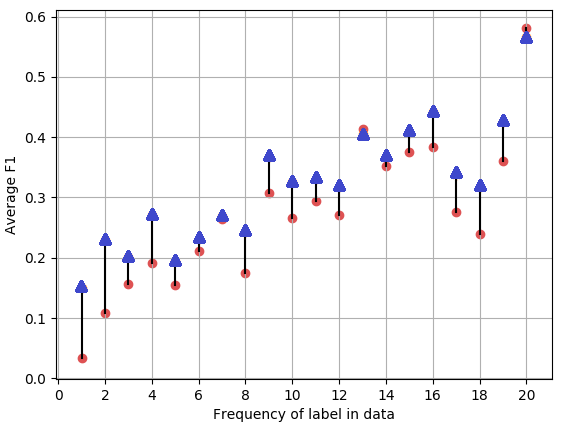
\includegraphics[width=0.5\columnwidth]{Images/labelf1_v2.png}
\caption{Average F1 over rare labels with the same frequency on TheGuardian dataset. Blue($\Delta$)=set-RNN, Red($\cdot$)=seq2seq-RNN.}
\label{fig:labelf1}
%\vspace{-6ex}
\end{figure}


\begin{figure}[t]
\centering
%\hspace{-2ex}
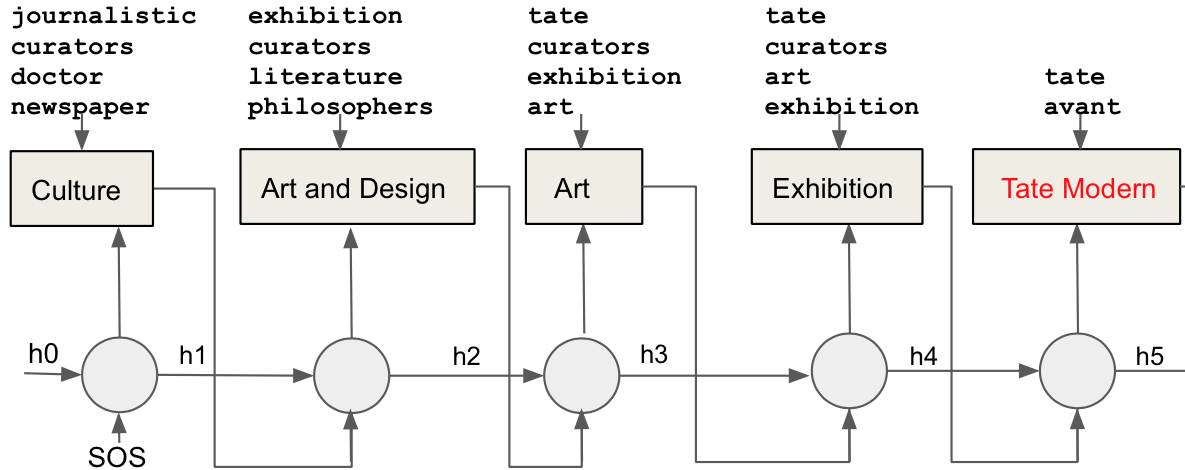
\includegraphics[width=0.8\columnwidth]{Images/train_sequence.png}
%\vspace{-4ex}
%\hspace{-2ex}
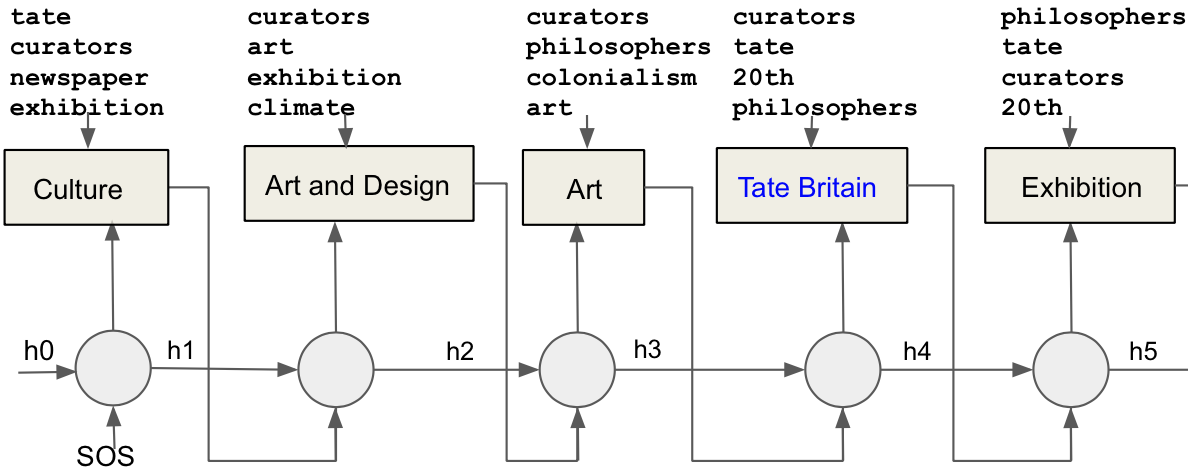
\includegraphics[width=0.8\columnwidth]{Images/train_set.png}

\caption{Top: best sequence by seq2seq-RNN; bottom: best sequence by set-RNN. Above models, at each time, we list the top unigrams selected by attention.}
\label{fig:models}
%\vspace{-6ex}
\end{figure}
We further demonstrate how latent label order helps in multi-label classification task with an example from TheGuardian\footnote{\scriptsize This document can be viewed at \url{http://www.guardian.co.uk/artanddesign/jonathanjonesblog/2009/apr/08/altermodernism-nicolas-bourriaud}}. Modeling label order as a latent variable relaxes the constraint that a model has to be trained in a given fixed label order. Figure~\ref{fig:models} shows the predictions made by standard RNN that simply mapping a label set to a sequence based on label frequencies (we will call this method seq2seq-RNN) and our method. In this particular example, the top sequence agrees with the top set in our method's prediction so we can just analyze the top sequence. seq2seq-RNN predicts \texttt{Tate Modern} (incorrect but more popular label) while we predict \texttt{Tate Britain} (correct but less popular label). The seq2seq predicted sequence is in the decreasing label frequency order while our predicted sequence is not. In the training data, \texttt{Exhibition} is more frequent than \texttt{Tate Britain} and \texttt{Tate Modern}. If we arrange labels by decreasing frequency, \texttt{Exhibition} is immediately followed by \texttt{Tate Modern} 19 times, and by \texttt{Tate Britain} only 3 times. So it is far more likely to have \texttt{Tate Modern} than \texttt{Tate Britain} after \texttt{Exhibition}. However, at the set level, \texttt{Exhibition} and \texttt{Tate Modern} co-occurs 22 times while \texttt{Exhibition} and \texttt{Tate Britain} co-occurs 12 times, so the difference is not so dramatic. In this case, imposing the sequence order biases the probability estimation and leads to incorrect predictions.
%We further demonstrate how set-RNN works with two examples. In the first example from the RCV1-v2 dataset, the most probable set predicted by set-RNN (which is also the correct set in this example) does not come from the most probable sequence. Top sequences in decreasing probability order are listed in Table~\ref{tab:pred_case_study}. The correct label set \{forex, markets, equity, money markets, metals trading, commodity\} has the maximum total probability of 0.161, but does not match the top sequence.